\section{Experiment Protocol}

\textbf{Project Title} \\
Evaluation of electrotactile feedback schemes in combination with myoelectric prosthetic control - closing the loop. 

\textbf{Information on Investigators} \\
The investigators are biomedical engineering Master students at Aalborg University. 

\textbf{Background} \\
Losing an upper limb can be hugely debilitating and can result in lowered quality of life due to restrictions in function, appearance and sensation. As a mean to regain the loss, transradial amputees can receive a functional prosthesis, where the majority are controlled by muscles signals, or electromyography (EMG). However, still 25\% of EMG prosthesis users reject their device, where a major reason for the low satisfaction is due to lack of sensory feedback.
Many advancements have been made in the academic community to improve function accuracy. However, combining function with sensory feedback, thus closing the motor/sensory loop, is still a scarcely investigated area. Therefore, this experiment will combine the control of a prosthesis with sensory feedback delivered via electrotactile stimulation electrodes placed on the forearm. During the experiment the subjects will test two different feedback configurations while controlling a virtual prosthesis, represented as a cursor on a computer screen.  

\textbf{Purpose} \\
The purpose of the experiment is to compare how subjects' perform in an evaluation test when receiving feedback from two different electrotactile stimulation configurations, respectively, in a closed loop virtual prosthesis. This might provide information on which feedback that seems more intuitive to use in practice in a prosthesis.


\textbf{Research Aim} \\
Test and evaluate two novel stimulation schemes, one based on modulating amplitude and one based on spatial localization of activation, for conveying sensory feedback of the prosthesis state in a closed loop prosthetic control system.

\textbf{Experiment Duration} \\
To be estimated.

\textbf{Inclusion Criteria} \\
The subject must be:
\begin{itemize}
	\item able bodied or transradially amputated as the highest degree of upper limb amputation.
	\item at least 18 years of age.
	\item able to understand, read and speak English and/or Danish.
	\item assessed by the investigators to comply with the instructions given during the experiment.
\end{itemize}

\textbf{Exclusion Criteria} \\
The subject must:
\begin{itemize}
	\item not have any diseases/conditions that may influence sensory perception.
	\item be willing to receive low amplitude current stimulation. 
\end{itemize}

\textbf{{\Large Experiment Procedure}} \\
\newline
The main focus of the experiment is for the subject to be able correctly interpret the two sensory feedback schemes. The grid illustrated in \figref{fig:gridmap} is the map the subject will be able to move around inside. Each square in the map will deliver a different stimulus corresponding to the motion state of the virtual prosthesis, represented as the black cursor. The square with center in the origin (square with cursor inside in \figref{fig:gridmap}) corresponds to resting state and will provide no sensory feedback. The remaining squares in the first row will deliver stimuli corresponding to only the wrist rotation degree of freedom (DOF), and the remaining squares in the third column will deliver stimuli corresponding to the closed hand DOF. The remaining squares will deliver a stimulation based on a combination of the two DOFs. The further away from resting state a square is, corresponds to a higher muscle contraction level.
The images located at each axis represent the hand movements needed to be performed to move the cursor in a desired direction. The control system will only react on one movement performed at a time. Thus, the cursor is only able to move along one axis at a time and not diagonally.

\begin{figure}[H]                 
	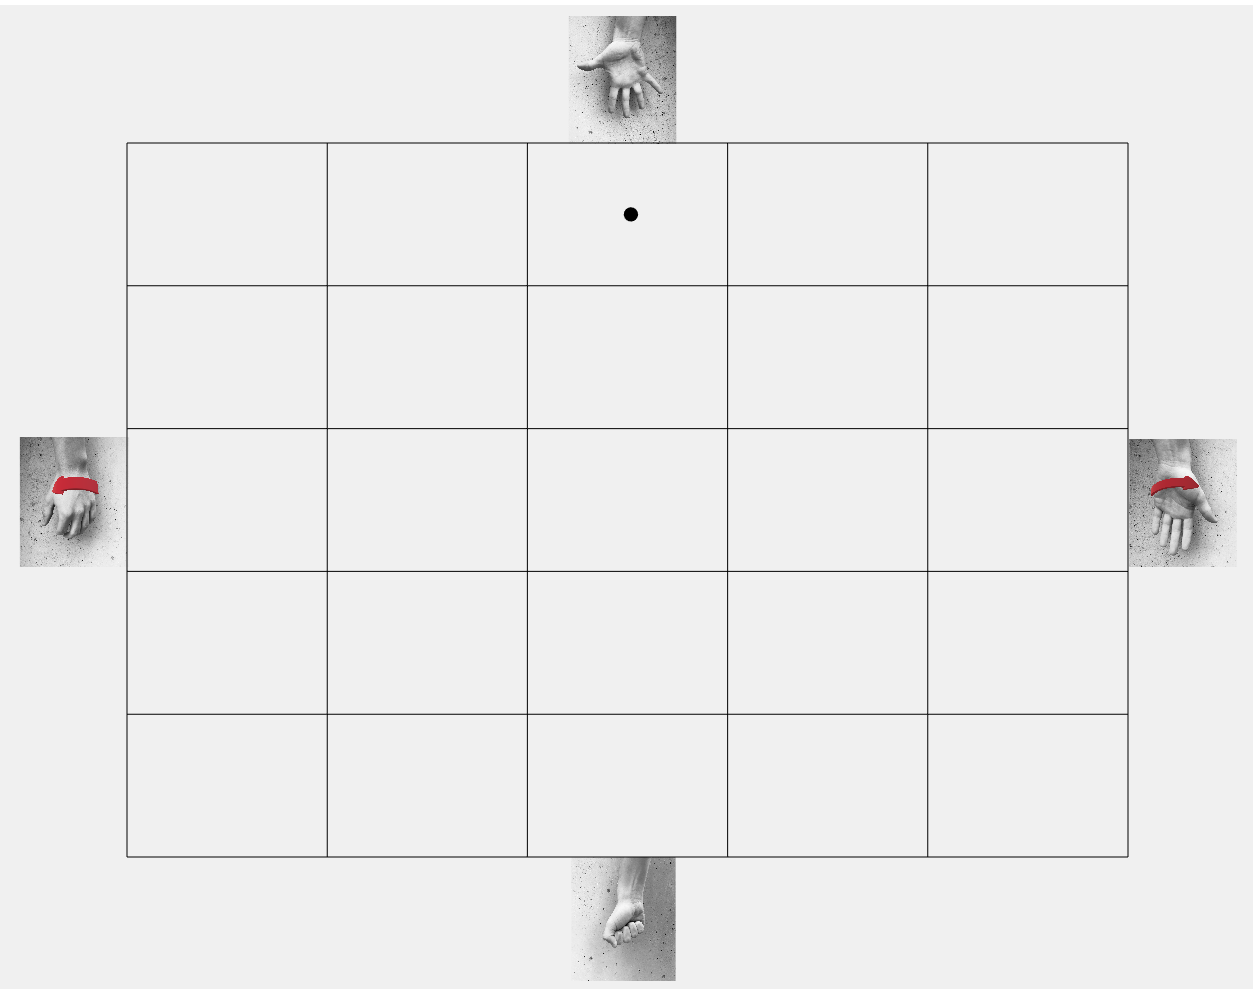
\includegraphics[width=0.78\textwidth]{figures/gridmap}  
	\caption{Image of the grid map and cursor used during all trainings and tests.}
	\label{fig:gridmap} 
\end{figure}

Before the final evaluation test is carried out the subject will be trained in controlling the cursor, trained in interpreting the sensory feedback and trained in interpreting the sensory feedback while controlling the cursor. The following order represent the chronology of the tasks the subject needs to undergo:

\begin{enumerate}
	\item Record EMG signals needed to build the prosthetic control system.
	\item Train the subjects ability to control the cursor via letting the subject move freely around inside the grid map.
	\item Perform target reaching test to evaluate the subject's ability to control the cursor.
	\item Record current amplitude thresholds needed to build the sensory feedback schemes.
	\item Train the subject's ability to interpret the single DOF sensory feedback of feedback scheme 1 by exposing the subject three times to each of the eight stimuli squares.
	\item Perform reinforcement learning on the eight squares from step 5 two times with sensory feedback from scheme 1.
	\item Perform validation test on the eight squares from step 5 two times with sensory feedback from scheme 1.
	\item Train the subject's ability to control the cursor while receiving sensory feedback from scheme 1 via letting the subject move freely around inside the grid map.
	\item Perform target reaching test where the cursor is invisible to evaluate how well the subject is to utilize the sensory feedback from scheme 1 regarding the cursor location.
	\item Redo step 5-9 with sensory feedback from scheme 2.
\end{enumerate}


\textbf{{\Large Hand Movements Used in the Experiment}} \\

\begin{figure}[H]                 
	\includegraphics[width=0.78\textwidth]{figures/handmovements}  
	\caption{Image of the hand movements used in the experiment. From top left corner: Wrist pronation, wrist supination, opened hand and closed hand.}
	\label{fig:handmovements} 
\end{figure}

\textbf{{\Large Experiment Setup}}

